\definecolor{g1}{RGB}{200 200 200}
\definecolor{g2}{RGB}{162 162 162}
\definecolor{g3}{RGB}{137 137 137}
\definecolor{g4}{RGB}{77 175 74}

% GNUPLOT: LaTeX picture with Postscript
\begingroup
  \makeatletter
  \providecommand\color[2][]{%
    \GenericError{(gnuplot) \space\space\space\@spaces}{%
      Package color not loaded in conjunction with
      terminal option `colourtext'%
    }{See the gnuplot documentation for explanation.%
    }{Either use 'blacktext' in gnuplot or load the package
      color.sty in LaTeX.}%
    \renewcommand\color[2][]{}%
  }%
  \providecommand\includegraphics[2][]{%
    \GenericError{(gnuplot) \space\space\space\@spaces}{%
      Package graphicx or graphics not loaded%
    }{See the gnuplot documentation for explanation.%
    }{The gnuplot epslatex terminal needs graphicx.sty or graphics.sty.}%
    \renewcommand\includegraphics[2][]{}%
  }%
  \providecommand\rotatebox[2]{#2}%
  \@ifundefined{ifGPcolor}{%
    \newif\ifGPcolor
    \GPcolorfalse
  }{}%
  \@ifundefined{ifGPblacktext}{%
    \newif\ifGPblacktext
    \GPblacktexttrue
  }{}%
  % define a \g@addto@macro without @ in the name:
  \let\gplgaddtomacro\g@addto@macro
  % define empty templates for all commands taking text:
  \gdef\gplfronttext{}%
  \gdef\gplfronttext{}%
  \makeatother
  \ifGPblacktext
    % no textcolor at all
    \def\colorrgb#1{}%
    \def\colorgray#1{}%
  \else
    % gray or color?
    \ifGPcolor
      \def\colorrgb#1{\color[rgb]{#1}}%
      \def\colorgray#1{\color[gray]{#1}}%
      \expandafter\def\csname LTw\endcsname{\color{white}}%
      \expandafter\def\csname LTb\endcsname{\color{black}}%
      \expandafter\def\csname LTa\endcsname{\color{black}}%
      \expandafter\def\csname LT0\endcsname{\color[rgb]{1,0,0}}%
      \expandafter\def\csname LT1\endcsname{\color[rgb]{0,1,0}}%
      \expandafter\def\csname LT2\endcsname{\color[rgb]{0,0,1}}%
      \expandafter\def\csname LT3\endcsname{\color[rgb]{1,0,1}}%
      \expandafter\def\csname LT4\endcsname{\color[rgb]{0,1,1}}%
      \expandafter\def\csname LT5\endcsname{\color[rgb]{1,1,0}}%
      \expandafter\def\csname LT6\endcsname{\color[rgb]{0,0,0}}%
      \expandafter\def\csname LT7\endcsname{\color[rgb]{1,0.3,0}}%
      \expandafter\def\csname LT8\endcsname{\color[rgb]{0.5,0.5,0.5}}%
    \else
      % gray
      \def\colorrgb#1{\color{black}}%
      \def\colorgray#1{\color[gray]{#1}}%
      \expandafter\def\csname LTw\endcsname{\color{white}}%
      \expandafter\def\csname LTb\endcsname{\color{black}}%
      \expandafter\def\csname LTa\endcsname{\color{black}}%
      \expandafter\def\csname LT0\endcsname{\color{black}}%
      \expandafter\def\csname LT1\endcsname{\color{black}}%
      \expandafter\def\csname LT2\endcsname{\color{black}}%
      \expandafter\def\csname LT3\endcsname{\color{black}}%
      \expandafter\def\csname LT4\endcsname{\color{black}}%
      \expandafter\def\csname LT5\endcsname{\color{black}}%
      \expandafter\def\csname LT6\endcsname{\color{black}}%
      \expandafter\def\csname LT7\endcsname{\color{black}}%
      \expandafter\def\csname LT8\endcsname{\color{black}}%
    \fi
  \fi
    \setlength{\unitlength}{0.0500bp}%
    \ifx\gptboxheight\undefined%
      \newlength{\gptboxheight}%
      \newlength{\gptboxwidth}%
      \newsavebox{\gptboxtext}%
    \fi%
    \setlength{\fboxrule}{0.5pt}%
    \setlength{\fboxsep}{1pt}%
\begin{picture}(5000.00,2500.00)%
    \gplgaddtomacro\gplfronttext{%
      \colorrgb{0.15,0.15,0.15}%
      \put(1000,2600){\makebox(0,0){\strut{}{\color{g4}{\rule[0.6mm]{0.5cm}{0.5mm}}} \footnotesize Output}}
      \put(2500,2600){\makebox(0,0){\strut{}{\color{g3}{\rule[0.6mm]{0.5cm}{0.5mm}}} \footnotesize $\mathcal{H}_1[\arg \min f_{\psi}^{\bm{M}}(\mathcal{H}_2)]$}}
      \put(3900,2600){\makebox(0,0){\strut{}{\color{g2}{\rule[0.6mm]{0.5cm}{0.5mm}}} \footnotesize $\mathcal{H}_1$}}
      \put(4500,2600){\makebox(0,0){\strut{}{\color{g1}{\rule[0.6mm]{0.5cm}{0.5mm}}} \footnotesize $\mathcal{H}$}}
      \put(468,250){\makebox(0,0)[r]{\strut{}\footnotesize $0.0$}}%
      \colorrgb{0.15,0.15,0.15}%
      \put(468,750){\makebox(0,0)[r]{\strut{}\footnotesize $0.25$}}%
      \colorrgb{0.15,0.15,0.15}%
      \put(468,1250){\makebox(0,0)[r]{\strut{}\footnotesize $0.50$}}%
      \colorrgb{0.15,0.15,0.15}%
      \put(468,1793){\makebox(0,0)[r]{\strut{}\footnotesize $0.772$}}%
      \colorrgb{0.15,0.15,0.15}%
      \put(468,2105){\makebox(0,0)[r]{\strut{}\footnotesize $0.928$}}%
      \colorrgb{0.15,0.15,0.15}%
      \put(468,2231){\makebox(0,0)[r]{\strut{}\footnotesize $0.991$}}%
      \colorrgb{0.15,0.15,0.15}%
      \put(500,30){\makebox(0,0){\strut{}\footnotesize $5$\texttt{e}-$05$}}%
      \colorrgb{0.15,0.15,0.15}%
      \put(970,30){\makebox(0,0){\strut{}\footnotesize $0.01$}}%
      \colorrgb{0.15,0.15,0.15}%
      \put(1576,30){\makebox(0,0){\strut{}\footnotesize $0.50$}}%
      \colorrgb{0.15,0.15,0.15}%
      %\put(2040,30){\makebox(0,0){\strut{}\footnotesize $10.0$}}%
      \colorrgb{0.15,0.15,0.15}%
      \put(2199,30){\makebox(0,0){\strut{}\footnotesize $27.86$}}%
    }%
    \gplgaddtomacro\gplfronttext{%
      \colorrgb{0.15,0.15,0.15}%
      \put(1349,-300){\makebox(0,0){\strut{}\footnotesize Outliers locational threshold $\delta_{\bm{l}}$ [m]}}%
    }%
    \gplgaddtomacro\gplfronttext{%
      \colorrgb{0.15,0.15,0.15}%
      \put(2893,250){\makebox(0,0)[r]{\strut{}\footnotesize $0.0$}}%
      \colorrgb{0.15,0.15,0.15}%
      \put(2893,750){\makebox(0,0)[r]{\strut{}\footnotesize $0.25$}}%
      \colorrgb{0.15,0.15,0.15}%
      \put(2893,999){\makebox(0,0)[r]{\strut{}\footnotesize $0.375$}}%
      \colorrgb{0.15,0.15,0.15}%
      \put(2893,1153){\makebox(0,0)[r]{\strut{}\footnotesize $0.452$}}%
      \colorrgb{0.15,0.15,0.15}%
      \put(2893,2137){\makebox(0,0)[r]{\strut{}\footnotesize $0.944$}}%
      \colorrgb{0.15,0.15,0.15}%
      \put(2925,30){\makebox(0,0){\strut{}\footnotesize $4$\texttt{e}-$05$}}%
      \colorrgb{0.15,0.15,0.15}%
      \put(3740,30){\makebox(0,0){\strut{}\footnotesize $\frac{\pi}{1000}$}}%
      \colorrgb{0.15,0.15,0.15}%
      \put(4114,30){\makebox(0,0){\strut{}\footnotesize $\frac{\pi}{100}$}}%
      \colorrgb{0.15,0.15,0.15}%
      \put(4749,30){\makebox(0,0){\strut{}\footnotesize $\pi$}}%
    }%
    \gplgaddtomacro\gplfronttext{%
      \colorrgb{0.15,0.15,0.15}%
      \put(3837,-300){\makebox(0,0){\strut{}\footnotesize Outliers angular threshold $\delta_{\alpha}$ [rad]}}%
    }%
    \put(0,0){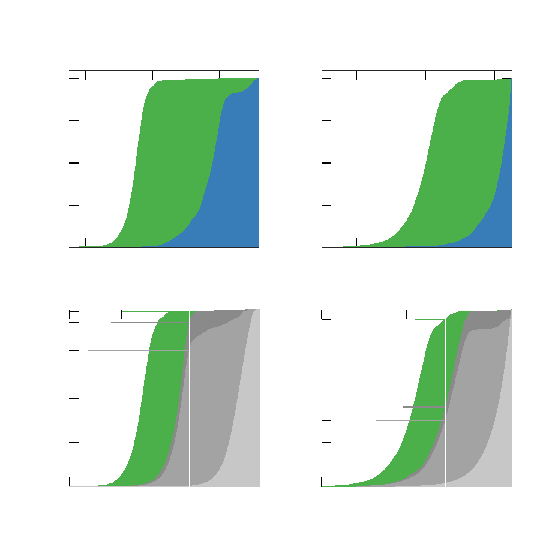
\includegraphics{./figures/experiments/a/awesomeness}}%
    \gplfronttext
  \end{picture}%
\endgroup
